\documentclass{math}

\usepackage{enumerate}
\usepackage{graphicx}

\title{Intro to Computer Science Theory: Homework 7}
\author{Alvin Lin and Joshua Cotton}
\date{August 2017 - December 2017}

\begin{document}

\maketitle

\subsection*{Problem 1}
For any alphabet \( \Sigma \), any nonnegative integer \( n \), and any
\( x_1,\dots,x_n\in\Sigma \), define \( d(x_1\dots x_n) \) as
\( x_1x_1\dots x_nx_n \). For instance \( d(aabab) = aaaabbaabb \). For
any language \( L \), define \( D(L) = \{d(x)\mid x\in L\} \) Show via
a formal construction FAs that if \( L \) is a regular language, then so
is \( D(L) \). Prove:
\[ \forall\text{FAs}~M(\exists\text{FA}~N(L(N) = D(L(M)))) \]


\subsection*{Problem 2}
Use the construction from Lemma 1.55 to make NFAs for the following REs. Your
NFAs should be the exact NFA that the construction would produce.
\begin{enumerate}[(a)]
  \item \( bab^*\cup b(ba\cup ab)^*bb \)
  \begin{center}
    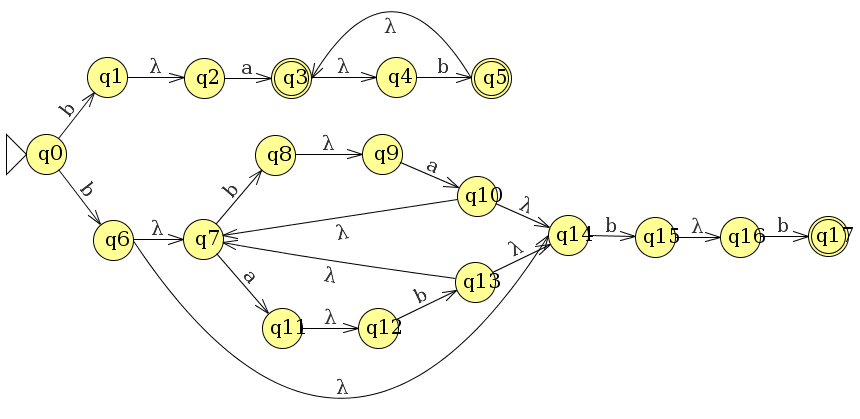
\includegraphics[width=16cm]{assets/hw_7_2a.png}
  \end{center}
  \item \( (a\cup b)(ab)^*(abb)^* \)
  \begin{center}
    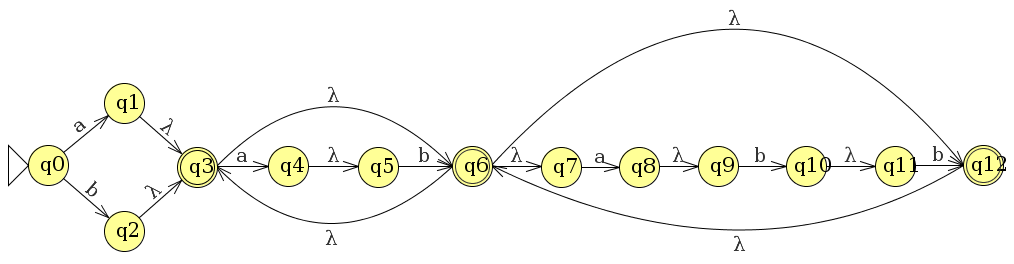
\includegraphics[width=16cm]{assets/hw_7_2b.png}
  \end{center}
\end{enumerate}

\subsection*{Problem 3}
Use the construction from Lemma 1.60 to make REs for the following DFAs. Your
resulting REs should be the exact ones that result from applying the
construction \textit{when you eliminate the states in numerical order}.
\begin{enumerate}[(a)]
  \item \( b^*aa^*\cup b^*aa^*b(ab^*aa^*b\cup ba^*b)^*ba^* \)
  \item \( a(a\cup b)\Bigg(\big((a\cup b)^2b\big)\cup\big((a\cup b)^2a(a\cup b)\big)\Bigg)^*
    (\epsilon\cup a\cup b) \)
\end{enumerate}

\begin{center}
  If you have any questions, comments, or concerns, please contact me at
  alvin@omgimanerd.tech
\end{center}

\end{document}
